% \documentclass[rnd]{mas_proposal}
\documentclass[thesis]{mas_proposal}

\usepackage[utf8]{inputenc}
\usepackage{amsmath}
\usepackage{amsfonts}
\usepackage{amssymb}
\usepackage{graphicx}
\usepackage{subcaption}

\renewcommand{\arraystretch}{1.5}
\newcommand{\cmark}{\ding{51}}%
\newcommand{\xmark}{\ding{55}}%

\title{Deep-Learning-Based Personalisation of Robot Behaviour for Assistive Robotics}
\author{Michał Stolarz}
\supervisors{Prof. Dr. Paul G. Plöger\\M.Sc. Alex Mitrevski}
\date{January 2023}

\thirdpartylogo{images/migrave.png}

\begin{document}

\maketitle

\pagestyle{plain}

\section[Introduction]{Introduction\footnote{Parts of this chapter have been published in~\cite{stolarz2022personalized,stolarz2022learningbased}}}

\subsection{Motivation}
One of the objectives of robot-assisted therapy (RAT)~\cite{esteban2017build} is increasing the autonomy of the robot that is used during therapy sessions; this has the purpose of reducing the necessary therapist interactions with the robot, while still keeping the therapist in control of the sessions at all times.
In the context of RAT, robot programs are usually developed in such a way that they can be used generically for different individuals; however, individuals may have different reactions to specific stimuli and, depending on their concrete needs, may also benefit from therapy sessions focusing on specific aspects.
This means that a generic RAT approach may not be optimal for effective treatment of individuals; instead, the robot should be able to adapt its behaviour to the needs of each individual and therapy session \cite{esteban2017build,scassellati2018improving,rudovic2018personalized}.

The motivation behind this work is a therapy for children with Autism Spectrum Disorder (ASD). This problem is of a big relevance as in the European Union, there are over 5 million people affected by autism~\cite{deenigma2022} and it is estimated that 1 in 160 children all over the world is diagnosed with ASD~\cite{jain2020modeling}. People with ASD often have difficulties in social interaction and communication. To alleviate the effects of ASD, individualized therapies are provided. However, autistic children find robots easier to communicate with than humans~\cite{robins2006}, thus Robot-Assisted Therapies (RATs) have been being investigated. During RAT, most of the time therapists have to control the robot remotely (Wizard of Oz approach)~\cite{deenigma2022}~\cite{david2018developing,robins2017developing,rudovic2017measuring,marinoiu20183d}. Because of it, the therapist might not be able to fully focus on the therapy and react appropriately to the child's behaviour~\cite{cao2018personalized}. To reduce their workload, the autonomy of the robot has to be increased, namely it should be able to interpret a child’s behaviour and adapt its actions to the individual needs of the child~\cite{esteban2017build}.

\subsection{Adaptation Techniques}
Adaptation is possible if the robot actively learns a user model that encodes certain attributes of the user. The user model can be integrated into a robot decision-making algorithm~\cite{rossi2017user} called a behaviour model, which allows the system to choose appropriate robot reactions in response to the actions of each individual user. Personalisation refers to the adaptation of the system to the individual user over time~\cite{rossi2017user} and can be solved by using Interactive Machine Learning (IML), which involves the user in the learning loop~\cite{senft2019teaching}. IML usually makes use of \emph{learning from guidance} or \emph{learning from feedback}. Learning from guidance relies on an external supervisor (e.g. therapist), who provides expert knowledge to the system. The supervisor is able to assess the decisions of the robot before being executed, namely they are able to accept, or alternatively reject and override the suggested reaction of the robot. This solution guarantees that the system will not execute any undesirable actions during learning, but is sensitive to the mistakes of the supervising person. On the other hand, learning from feedback uses direct feedback from the user (e.g. engagement level of the user). As there is no supervising person, the robot has to explore by itself what effects its actions have. 

\subsection{Problem Statement}
The main problem during RAT for children with autism is that the therapists have to control the robot manually, which might meaningfully increase their workload. This means that there is a need for a personalised behaviour model which will increase the autonomy of the robot. The model should interpret and continuously adapt to the behaviour of the individual child under therapy, as each child might have different ASD symptoms. The therapy for children with ASD usually consists of games designed by the therapists. This means that the developed learning algorithm should be able to enable the robot to personalise the difficulty of the game activities to the individual child's skill level. Additionally, the robot should also react appropriately when interacting with the child does not go as planned. That means that the robot should prevent them from getting bored, disengaged or demotivated, by executing actions such as giving verbal motivating feedback or simple motions (e.g. waving gesture) that would draw the child’s attention back to the game.

Currently, in order to enable the robot to react appropriately in various social situation during an interaction with the user, many works make use of an engagement estimator. Engagement is the feature that is often used for the development of behaviour models~\cite{senft2015sparc,senft2015human,tsiakas2018task,del2022learning}. It can be measured with the use of EEG headset~\cite{tsiakas2018task}, but an external engagement observer might be more convenient for children with ASD, as they may be overwhelmed by the sensory stimuli if they need to wear an additional device during therapy~\cite{javed2019robotic}. In the literature, several types of algorithms that estimate engagement from features obtained using the OpenFace library~\cite{baltrusaitis2018openface, jain2020modeling, kaur2019domain, karimah2021implementation}, eye gaze~\cite{khorrami2014system},  body posture~\cite{ritschel2017adapting} or visual data~\cite{mane2018engagement, del2020you} can be found. Some of these are also able to capture and classify temporal data~\cite{del2020you, karimah2021implementation}.

However, the model estimating an engagement used further for decision-making process is not perfect and might introduce an additional error to the behaviour model. This is a problem of a significant impact on the robot behaviour and was mentioned in our recent work~\cite{stolarz2022learningbased}. To alleviate the impact of false predictions on the feature level we suggest to turn towards data-driven methods that will be able to use a raw sensor data instead of high-level features (e.g. engagement level) that have to be estimated separately. However, the tabular approaches like Q-learning (used in our recent work~\cite{stolarz2022learningbased}), are unsuitable for big state spaces~\cite{akalin2021reinforcement}, like raw sensory data. That is why in this work, we are planning to use deep learning (DL) for that purpose. In the next section, we will introduce DL techniques used in the context of decision-making for social robotics.


\section[Related Work]{Related Work\footnote{Parts of this chapter have been published in~\cite{stolarz2022personalized}}}

As we discussed in~\cite{stolarz2022personalized}, there are four personalisation approaches that are provided in the context of HRI, namely: social behaviour, game difficulty, affective, and user preferences (e.g. proxemics) personalisation. However, the main focus should be put on two first personalisation techniques. The DL has been explored in the field of the social behaviour personalisation and game difficulty personalisation. The latter, however, refers more to the agent not as a tutor but as an opponent in the game.

\subsection{Deep Learning Personalisation Approaches}

\subsubsection{Social Behaviour Personalisation}
Qureshi et al~\cite{Qureshi2016} made a step towards making robots more interactive while coexisting with humans. This is done by enabling the robot to continuously learn social interaction skills. For that purpose, the deep reinforcement learning (DRL) method was used, which is called Multimodal Deep Q-Network (MDQN)\footnote{The original implementation is available under \url{https://github.com/ahq1993/Multimodal-Deep-Q-Network-for-Social-Human-Robot-Interaction}}\footnote{The python implementation (used in~\cite{Belo2021}) is available under \url{https://github.com/JPedroRBelo/pyMDQN}}, which is based on DQN~\cite{mnih2015human}. This is a major contribution, as the developed DRL interaction model can conduct a human-robot interaction in an uncontrolled and real environment, which is not the case for the previous works. There are two inputs for MDQN, namely grayscale and depth video frames. Based on these two streams the model learns when to perform one of the four actions, which are: \emph{wait}, \emph{look towards human}, \emph{wave hand}, \emph{handshake}. The reward function is designed such that the robot's main goal is to perform a successful handshake. Here the data generation and training phases are separated, which means that all the robot's experiences are saved in the replay memory and used for training only during the resting period. 

In~\cite{Qureshi2017} the MDQN model was augmented by adding a recurrent attention model~\cite{sorokin2015deep} in order to enable the network to focus on certain fragments of the input data. This approach was proven to increase people's willingness to interact with a robot (through handshaking). However, the new model requires more training data in order to reach performance of the neural network without attention. There are three deficits of the aforementioned approaches which are related to deploying the robot in the real environment. Firstly, the action space consists only from four actions, which might be insufficient for reacting to human behaviour in real life. Secondly, the designed reward function is task-specific and may be difficult to adjust to different applications (here handshaking is rewarded explicitly); it should be mentioned as well that external rewards are scarce and might make learning relatively slow. Moreover, as training the neural network is computationally heavy, it has to be performed during the robot resting period, as otherwise it could cause delays during the interaction period. This is a significant disadvantage, which implies that the policy is not updated continuously during an interaction, which may cause a user to be disengaged. 

In the follow-up work~\cite{Qureshi2018}, the authors faced the second deficit and proposed an intrinsically motivated DRL. The internal reward, used for training the Deep Q-network (Fig.~\ref{fig:mdqn}), is calculated with the use of an action-conditional prediction network (Pnet) as an error between Pnet's event prediction and detected event occurrence. The aforementioned events are an observed behaviour of the interacting partner, such as handshake, eye contact and smile. It is moreover shown that intrinsically motivated DRL leads to more human-like behaviour than DRL based on an external reward. However, during the experiments it was noticed that the robot was repeating a handshake action even after already successful handshake. This behaviour may be unusual from the perspective of the normal person and should be avoided (e.g. with memory and by preventing the robot from being oblivious).

\begin{figure}[htb!]
	\centering
	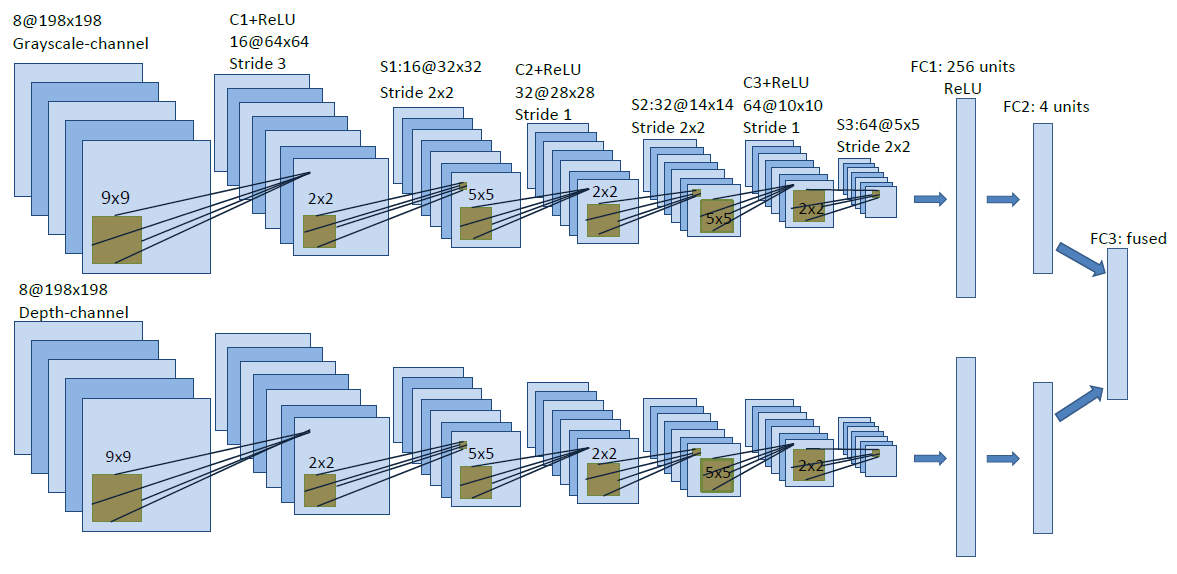
\includegraphics[width=0.7\textwidth]{images/architecture/mdqn.png}
	\caption{Architecture of the Deep Q-Network~\cite{Qureshi2018}}
	\label{fig:mdqn}
\end{figure}

Belo et al~\cite{Belo2022} also made an approach to make robots more socially acceptable and natural while interacting with humans. For that purpose the Social Robotics Deep Q-Network (SocialDQN) was developed, which is based on the MDQN architecture. However, in SocialDQN the input for the depth information was substituted with the input indicating the emotional state of the user with Ekman's six basic emotions~\cite{ekman1971constants}: \emph{fear}, \emph{happiness}, \emph{disgust}, \emph{anger}, \emph{sadness}, \emph{surprise}. The authors conducted tests in the developed simulator~\cite{Belo2021} where the 13 human referees had to assess if the robot performed correct actions in each of the considered scenarios. In the end three models were compared, namely a random policy action selector, SocialDQN with and without social signals as an extra input. It was shown that SocialDQN, considering social signals, outperforms the two other predictors. It reached an accuracy of 89.50\%. Unfortunately, no comparative study was performed with an original MDQN. Moreover, the evaluation was performed only in the simulation and not during a real-life interaction with a real human. Another deficit is that the action space of SocialDQN is relatively small as it consists of only four actions (similarly to MDQN).
 
Clark-Turner et al~\cite{ClarkTurner2017} aim at developing a framework enabling the robot to deliver a behavioural intervention (BI). The idea behind BI is to teach children with certain disorders to perform new behaviours. The authors used for that purpose deep recurrent Q-network (DRQN) which is trained from human demonstrations. This is a major contribution as no previous work used DRQN to learn human policy for choosing discrete actions based on the demonstration data. There are two inputs for the developed model, namely: RGB image, point cloud and an audio spectrogram. The set of possible actions consists of: \emph{command}, \emph{prompt} (in both cases the robot waves and greets the user, with an exception that the latter provides also a prompt saying what is expected from the participant), \emph{reward} (giving a positive appraisal to the user followed by ending the session by saying goodbye), \emph{abort} (ending the session when the user's response is negative consequently). The reward for the robot is positive whenever the actions are performed correctly, otherwise no reward is provided. Unfortunately, no real-life tests were conducted as the proposed algorithm was evaluated only with the collected demonstration data, where the robot was tele-operated. Moreover, the obtained results show a relatively small accuracy of the model (43.2\%-83.3\%) which may be insufficient for deploying it for the real behavioural intervention.

Both of the aforementioned deficits were faced in the next work of the same authors~\cite{Turner2018}. First of all, the approach to increase a model's accuracy with transfer learning was made. It means that the network extracting features from the RGB data was a IRNV2 network pre-trained on the ImageNet. Additionally, the used modalities were changed, namely a point-cloud was replaced with an optical flow image. Unfortunately, no comparative evaluation between an old and new approach was performed, so the improvement of the introduced changes can not be directly shown. However, the authors faced the second deficit and performed not only evaluation on the collected dataset but also a real-life tests. The reported accuracy in both cases was not exceeding 80\%. Moreover, the authors limited the number of actions to three, namely: \emph{PMT}, \emph{REW}, \emph{END} (which correspond to \emph{prompt}, \emph{reward} and \emph{abort} respectively).

In~\cite{Romeo2018} the goal of the authors is to develop the robot that would accompany the elderly. For that purpose the authors developed a multimodal system that can make a decision on how and with whom it should start an interaction. There are two contributions of this work, namely, collection of the dataset focusing on initiation of the interaction and training a convolutional neural network (CNN) on it. The data was collected in two sessions, during the first one single users were interacting with the robot and during the second one two participants were acting in front of the robot. The aforementioned CNN was trained and evaluated on the collected dataset. The input of the network consists of the grayscale images and the output of three actions: \emph{waiting}, \emph{calling for attention} (waving and introducing), \emph{starting the interaction} (asking a direct question). The reward  was designed to be positive or 0 in case of the correct use of the action and negative otherwise. The deficit of that work is that the trained CNN was evaluated only on the dataset (not in the real-life interaction) and the limited action space (only three actions). However, the reported accuracy is promising as it reached 93\%. 

In the next work~\cite{Romeo2018}, Romeo et al faced one deficit of~\cite{Romeo2018} and evaluated the model during a real-life tests that lasted for four days. To improve the models capabilities, at the end of each day, the network was fully retrained (including the new data). According to the reported results, the accuracy of the network, obtained on the updated dataset was still 93\% at the end of the last experimentation day. However, the accuracy of the CNN, obtained during an actual interaction with the study participants and calculated as number of correctly chosen actions accordingly to the participants opinions, was 44\%, 58\%, 56\% and 59\% (each one obtained on each single day). The additional details of the conducted experiments and the model can be found in~\cite{romeo2021human}.

Hijaz et al directly approached the problem of increasing autonomy of the robot used during the therapies for individuals with ASD~\cite{Hijaz2021}. The authors propose a system for learning the therapist's verbal behaviour during the intervention delivery through Learning from Demonstration (LfD). There are two contributions of the aforementioned work. Firstly, in the other works the collected data used for training the model is collected in a simulation~\cite{Turner2018,Belo2021,Belo2022} or laboratory environment~\cite{ClarkTurner2017,Turner2018,Romeo2018} which usually simplifies real-world interaction. In this work however, the data was collected in a clinical setting, during a real intervention, where the robot was tele-operated by a therapist. Secondly, in the previous works the actions delivered by the robot were pre-scripted which is the cause of the learned behaviour being unnatural in the end. In~\cite{Hijaz2021} the actions were taken directly from the demonstrations given by therapists (as the robot was tele-operated during the intervention). The input to the used deep neural network (DNN) model was a child audio spectrogram and last therapist behaviour. The action space is relatively big in comparison to other works~\cite{Qureshi2016,Qureshi2017,Qureshi2018,ClarkTurner2017,Turner2018,Belo2021,Belo2022,Romeo2018,Romeo2019} as it consists of 9 actions, namely: saying that the robot is in one of six emotional states (angry, surprised, tired, scared, happy, sad), discriminative stimulus (asking the child how the robot is feeling followed by emotion presentation using body language), social praise (in case the child gives a correct answer during a game) and random actions (used to maintain child's engagement). There main deficit of the presented work is a very low accuracy (43.48\%), which might be due to insufficient amount of collected data which was additionally imbalanced. Moreover, the system was not tested in the real-life scenario, but only on the collected dataset. 


\subsubsection{Game Difficulty Personalisation}
When it comes to game difficulty personalisation, the DL algorithms were used so far as opponent players in the board/computer games. In~\cite{Silver2016} the authors managed to develop the algorithm (based on deep neural network) that was able to defeat a professional player in the game of Go. The DQN was proved to achieve a performance of professional games testers~\cite{mnih2015human}. In~\cite{hausknecht2015deep} the authors added Long Short-Term Memory (LSTM)~\cite{hochreiter1997long} layer in order to enable DQN to remember distant events. In~\cite{sorokin2015deep}, the authors managed to improve the performance of DQN by adding an attention mechanism, which also increased an interpretability of the network decisions (ability to determine on which regions of the image the network is focusing). 

Finally, in the robotics field, in~\cite{Cuayahuitl2017}, the author designed another variant of DQN which was further deployed on the conversational robot playing the \emph{Tic-tac-toe} game. The main aim of the work was to develop a humanoid robot that would play games with people having a brain illness, and thus slow down their decline. The deployed model is an improvement to the previous work as it provides not only game difficulty but also social behaviour personalisation. The robot is able to play the game with the user, as well as perform certain dialogue acts. In total the action space is relatively big as it provides 18-34 actions (depending on the size of \emph{Tic-tac-toe} grid), consisting of dialogue acts (speech and arm movements) and games moves. The state space consist of the features describing the game moves and words that occurred during an interaction. The authors evaluated the system with the user simulation (with semi-random behaviour). The results indicate that the system was able to conduct successful interactions and the proposed variant of DQN obtains higher winning rates than the original DQN.

The deficit of~\cite{Cuayahuitl2017} was faced in~\cite{Cuayahuitl2020} where the authors performed a real world evaluation. The proposed variant of DQN (in~\cite{Cuayahuitl2020} extended to two variants of \emph{Tic-tac-toe} game) was tested with 130 study participants for four nonconsecutive days in-the-wild (outside of the laboratory environment). The authors reported that the users were impressed  with the robot, however no quantitative nor qualitative measures were provided.

However, all of the aforementioned works describe DRL agent as an opponent playing a game against a human user. No solutions for DRL just choosing the game difficulty for the user were found. Akalin et al~\cite{Akalin2018} proposed an initial idea for a DRL for adjusting the difficulty level of the game during a social human-robot interaction with elderly people. According to the authors, the input would consist of three variables, namely, user's valence and engagement, as well as state of the game (the last difficulty level and information if the game is stopped or paused). The action space would consist of five actions: increasing, decreasing, not changing a difficulty level or pausing or stopping the game. The reward would be calculated based on valence and engagement of the user. Unfortunately,~\cite{Akalin2018} is just a proposal of the solution without any implementation details nor results. 

\subsection{Available Datasets}
 For training a DL agents a huge amount of data is required, which explains a necessity for a dataset. We looked for publicly available datasets that can be used for training DL decision-making agents. Unfortunately, all of them can only be applied for testing a feasibility of social behaviour personalisation models. Because the datasets contain visual data we categorised them into two groups, depending on the perspective of the camera from which the video/pictures were recorded. The following datasets contain data recorded from the first-person perspective (the human partner/s is/are directly interacting with the robot):
\begin{itemize}
	\item AIR-Act2Act~\cite{Ko2021}: 100 subjects, 10 actions, 5000 samples, 3 modalities (depth, skeleton, RGB)
	\item NTU RGB+D~\cite{Shahroudy_2016_CVPR,Liu2020}: 106 subjects, 26 actions, 8276 samples, 3 modalities (depth, skeleton, RGB).
	\item \cite{ryoo2013firstperson}: 8 subjects, 7 actions, 684 samples, 1 modality (RGB) 
	\item \cite{ryoo2015robot}: 8 subjects, 9 actions, 180 samples, 2 modalities (RGB, depth)
	\item AUTH UAV Gesture~\cite{patrona2021overview} (contains parts of datasets presented in \cite{Shahroudy_2016_CVPR,Perera_2018_ECCV_Workshops}): 8 subjects (newly captured), 6 actions, 4930 samples, 1 modality (RGB) 
\end{itemize}

Most of the aforementioned datasets are designed for activity recognition~\cite{Shahroudy_2016_CVPR,Liu2020,ryoo2013firstperson}, activity prediction~\cite{ryoo2015robot} and gesture recognition~\cite{patrona2021overview}. Only the AIR-Act2Act~\cite{Ko2021} dataset was designed with the purpose of teaching the robot social skills, namely the scenario, where the study participant is performing an action, is labeled with the reaction type that the robot should undertake. Additionally, this dataset contains the robot behaviours (body gestures) that should be performed as a reaction. None of the aforementioned datasets can be used for training the model that would be applicable for ASD therapy. However, they can be used for checking a feasibility of the DL architecture (e.g. MDQN) that can be further trained in the simulation or on the manually collected dataset. Unfortunately, only certain datasets are easily available online, namely: AIR-Act2Act, AUTH UAV Gesture, NTU RGB+D.

\begin{figure}[htb!]
	\centering
	\begin{subfigure}[b]{0.22\textwidth}
		\centering
		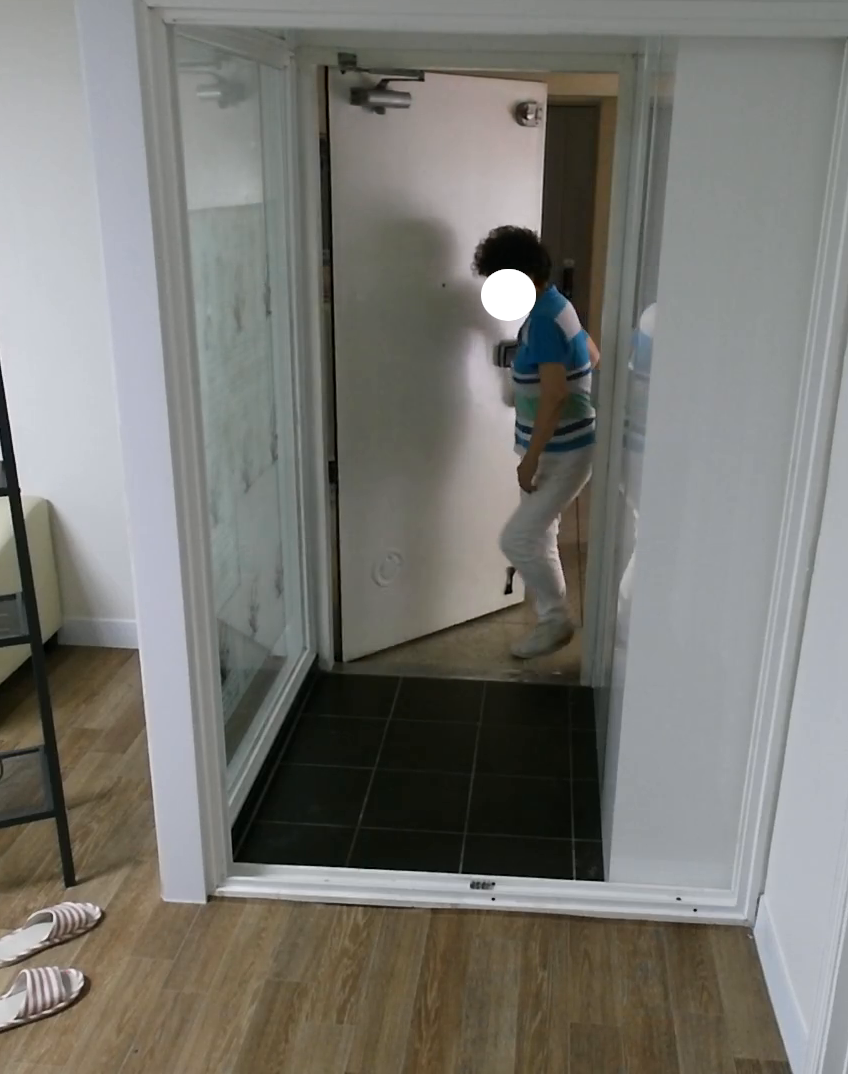
\includegraphics[width=0.9\textwidth]{images/dataset/1.png}
		\subcaption{}%
		\label{subfig:normal_1}
	\end{subfigure}
	\begin{subfigure}[b]{0.22\textwidth}
		\centering
		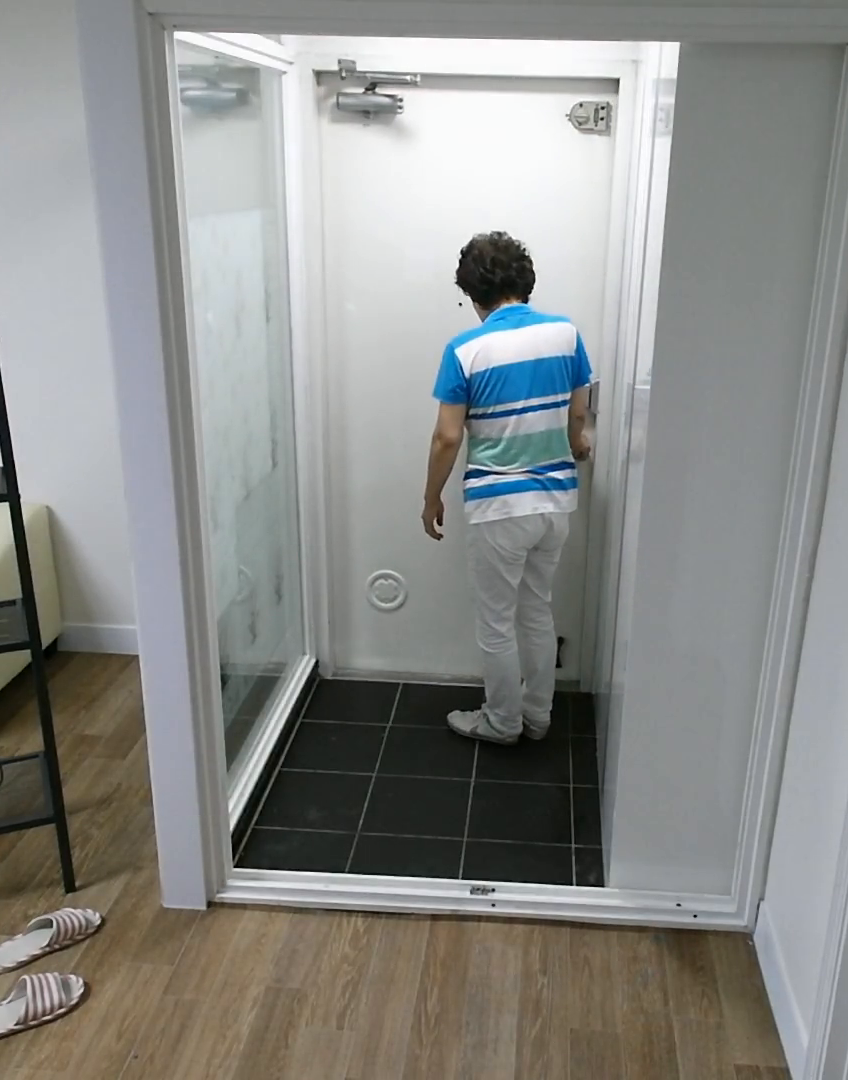
\includegraphics[width=0.9\textwidth]{images/dataset/2.png}
		\subcaption{}%
		\label{subfig:left}
	\end{subfigure}
	\begin{subfigure}[b]{0.22\textwidth}
		\centering
		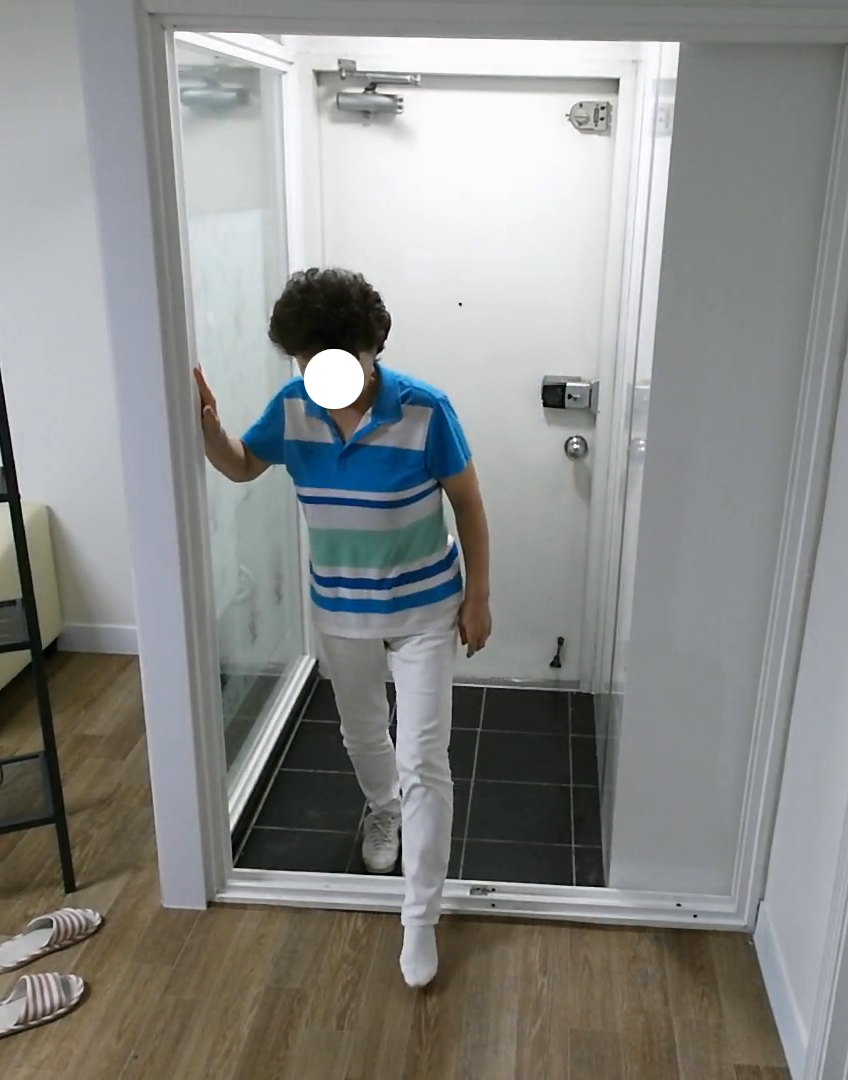
\includegraphics[width=0.9\textwidth]{images/dataset/3.png}
		\subcaption{}%
		\label{subfig:both_apart}
	\end{subfigure}
	\begin{subfigure}[b]{0.22\textwidth}
		\centering
		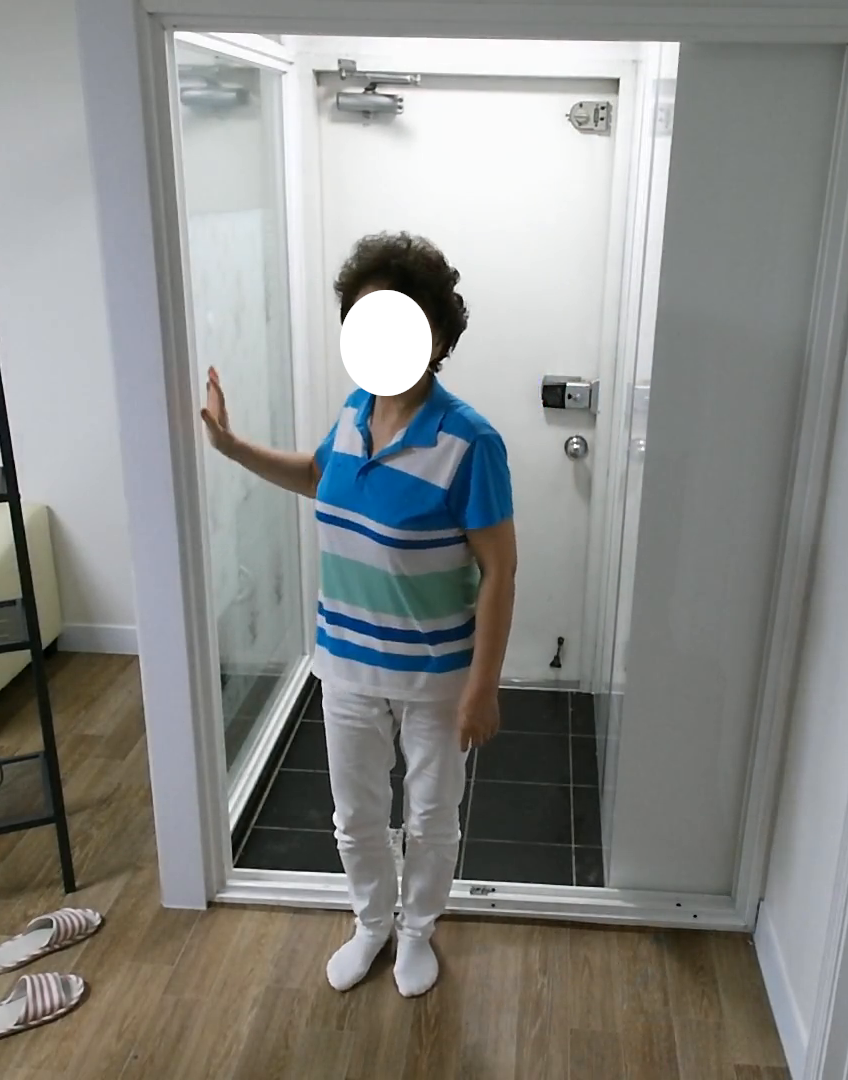
\includegraphics[width=0.9\textwidth]{images/dataset/4.png}
		\subcaption{}%
		\label{subfig:right}
	\end{subfigure}
	\caption{Frames (preprocessed) from one of the videos from AIR-Act2Act dataset~\cite{Ko2021} (the video depicts a scenario where the robot is supposed to bow to the elderly person who enters into the apartment)}
	\label{fig:hoora}
\end{figure}

The requirement for using a certain dataset are recordings from the first-person perspective (the person participating in the interaction). That is why the datasets containing recordings with only the perspective of the third person (two people are interacting with each other and the robot is only an observer)~\cite{Hu2013,UT-Interaction-Data,Gemeren2016,Yun2012} are unsuitable for our application.

\subsection{Tools for Data Collection}

As mentioned before, the provided datasets are not suitable for training the model that would be applicable for ASD therapy. That is why during the project it will be required to collect the dataset manually or in the simulation. In both cases the data will not be collected from the individuals with authism, however the scenarios imitating an robot-conducted intervention can be replicated with people without autism (students and university staff) or with simulated users. For both cases there are available tools that can be reused in the proposed project. 

First of all, the autism intervention scenarios can be simulated with the Simulator for Deep Reinforcement Learning and Social Robotics (SimDRLSR)~\cite{Belo2021}.\footnote{\url{https://github.com/JPedroRBelo/simDRLSR}} Here, the actions of the simulated humans are defined with scripts. Additionally, the robot's actions can be evaluated (whether they are socially acceptable) by human referees with a provided validation tool~\cite{Belo2022}\footnote{\url{https://github.com/JPedroRBelo/validation_tool_socialdqn}}. Although a simulation is a cheap and fast method for data collection for training a DL agent, the important features for action selection during an autism intervention are facial expressions, eye gaze and head orientation of the users~\cite{stolarz2022learningbased}, which might not be possible to reflect in the simulation.

Another possibility is to collect the data manually. This requires a suitable software that would enable a researcher to control the robot, as well as appropriately organise and store the collected data. There are publicly available packages that can be used as a guideline for creating such a software~\cite{Turner2018,carpio2018learning,carpio2019learning}\footnote{\url{https://github.com/AssistiveRoboticsUNH/deep_reinforcement_abstract_lfd}}\footnote{\url{https://github.com/AssistiveRoboticsUNH/TR-LfD}}.

\section{Problem Statement}
\begin{itemize}
    \item Which of the deficits are you going to solve?
    \item What is your intended approach?
    \item How will you compare you approach with existing approaches?
\end{itemize}

\section{Project Plan}

\subsection{Work Packages}
\emph{Planning is the replacement of randomness by error.} (Einstein). Very much like you would never start a longer journey without a detailed travel plan, you should not start a project without a carefully though out work plan. A work package is a logical decomposition of a larger piece of work into smaller parts following a ``divide and conquer" strategy. It is very specific to the problem that you are going to address. Refrain from a rather generic decomposition. If your work plan looks similar to those of your school mates, which may address completely different problems then you have not thought carefully enough about how you approach the problem. It is ok to have two generic work packages \emph{Literature Study} and \emph{Project Report}. Discuss your work packages in the ASW seminar.

The bare minimum will include the following packages:
\begin{enumerate}
    \item[WP1] Literature Study
    \item[WP2] ...
    \item[WP3] ...
    \item  ...
    \item[WPy] Evaluation of approach and comparison with similar approaches
    \item[WPz] Project Report
\end{enumerate}

\subsection{Milestones}
Milestones mark the completion of a certain activity or at least a major achievement in an activity. Milestones are also decision points, where you reflect on what you have achieved and what options you have for continuing your work in case you have not achieved what was planned. Above all, milestones have to be measurable. As above, if your milestones are the same as those of your school mates, then you may not have thought carefully enough about how your project shall progress.
\begin{enumerate}
    \item[M1] Literature review completed and best practice identified
    \item[M2] ...
    \item[M3] ...
    \item[M4] Report submission
\end{enumerate}

\subsection{Project Schedule}
Include a Gantt chart here. It doesn't have to be detailed, but it should include the milestones you mentioned above.
Make sure to include the writing of your report throughout the whole project, not just at the end.

\begin{figure}[h!]
    \includegraphics[width=\textwidth]{images/rnd_deliverable_timeline}
    \caption{My figure caption}
    \label{fig:myfigure}
\end{figure}

\subsection{Deliverables}

\subsubsection*{Minimum Viable}
\begin{itemize}
    \item Project results required to get a satisfying or sufficient grade.
\end{itemize}

\subsubsection*{Expected}
\begin{itemize}
    \item Project results required to get a good grade.
\end{itemize}

\subsubsection*{Desired}
\begin{itemize}
    \item Project results required to get an excellent grade.
\end{itemize}

Please note that the final grade will not only depend on the results obtained in your work, but also on how you present the results.

\nocite{*}

\bibliographystyle{plainnat} % Use the plainnat bibliography style
\bibliography{bibliography.bib} % Use the bibliography.bib file as the source of references

\end{document}
